\documentclass[12pt]{article}

%setup
\usepackage{setspace}
\usepackage{graphicx}
\usepackage{amsmath}
\usepackage{datetime}
\usdate
\usepackage{enumitem}
\usepackage[bottom]{footmisc}
\interfootnotelinepenalty=10000
\usepackage{subfigure}
\usepackage{hyperref}
\usepackage{float}
\usepackage{placeins}
\usepackage{chngpage}
\usepackage[margin=1in]{geometry}
\hypersetup{
    colorlinks = true,
    urlcolor = cyan,
    citecolor = cyan,
    linkcolor = cyan
}
\usepackage[backend=biber,style=apa,autocite=inline]{biblatex}
\usepackage{lscape}
%\DeclareLanguageMapping{english}{english-apa}
\addbibresource{paper.bib}
\setcounter{tocdepth}{2}

%\addtolength{\oddsidemargin}{-.875in}
%\addtolength{\evensidemargin}{-.875in}
%%\addtolength{\textwidth}{1.75in}
%\addtolength{\topmargin}{-.875in}
%\addtolength{\textheight}{1.75in}

\begin{document}
%\setlist{noitemsep}

\newcommand{\tit}{International Financial Entanglement: U.S. Monetary Policy and Bond Spreads in Emerging Markets}

\newcommand{\ack}{Final draft of term paper for AEM 4545: International Finance and Macroeconomics, taught by Professor Eswar Prasad in Fall 2019.}

\newcommand{\abs}{\noindent Economists have frequently questioned the extent of the linkages between advanced economies and  emerging market economies (EMEs). Yet, the literature and theory have thus far not determined the direction and extent of these linkages for monetary policy in the post-Great Recession era. I test the relevance of U.S. monetary policy in driving changes in EMEs in a regression framework with fixed effects and country specific models. Yield spreads in emerging markets are compared to the federal funds rate, controlling for a country-specific economic conditions, economic characteristics, fiscal conditions, international market strength, and global uncertainty. I use panel data across 16 EMEs spanning 20 years, finding evidence that U.S. monetary policy plays a significant role in determining financial market conditions when pooling data; additionally, U.S. monetary policy has significant effects in determining financial market conditions for specific countries. I also investigate time-based interaction effects for the federal funds rate and the 2013 Taper Tantrum, recessions, and the Great Recession of 2007-09. The effects point to evidence against increased financial decoupling, suggesting that global factors still determine the movement of sovereign bond spreads.
}

\title{\tit{\thanks{\ack}}}

\author{Darren Chang}
\date{{\today}}

\maketitle
\thispagestyle{empty}

\begin{abstract}
  \abs  
\end{abstract}

\newpage
\setcounter{page}{1}

% Print table of contents
%    \begin{singlespacing}
%    \tableofcontents
%    \end{singlespacing}
%    \clearpage

\section{Introduction}
Investors, academics, and central bankers all appreciate stable and definitive models of market reactions to central banking policy. But, central banking effects have eluded precise predictions. This is especially the case for EMEs, which have diverse characteristics and inconsistent mechanisms for market movements.

After an extended period of heightened volatility during and after the 2007-09 Great Recession, EME sovereign spreads decreased in 2010, with occasional spikes in 2012 and 2015 only for the Europe, Middle East, and Africa (EMEA) region (Figure~\ref{fig:globalfx}). The emerging market trends mirror the reaction of the U.S. bond spreads, albeit with changes of lower magnitude due to the intrinsically higher premia demanded for assets in riskier EMEs. The strength of the global market was portended by high certainty over monetary policy and high liquidity coupled with low yields, especially in the United States~\parencite{csonto13}.
\begin{figure}[h!]
\caption{Global Effects of U.S. Central Banking}
\centering
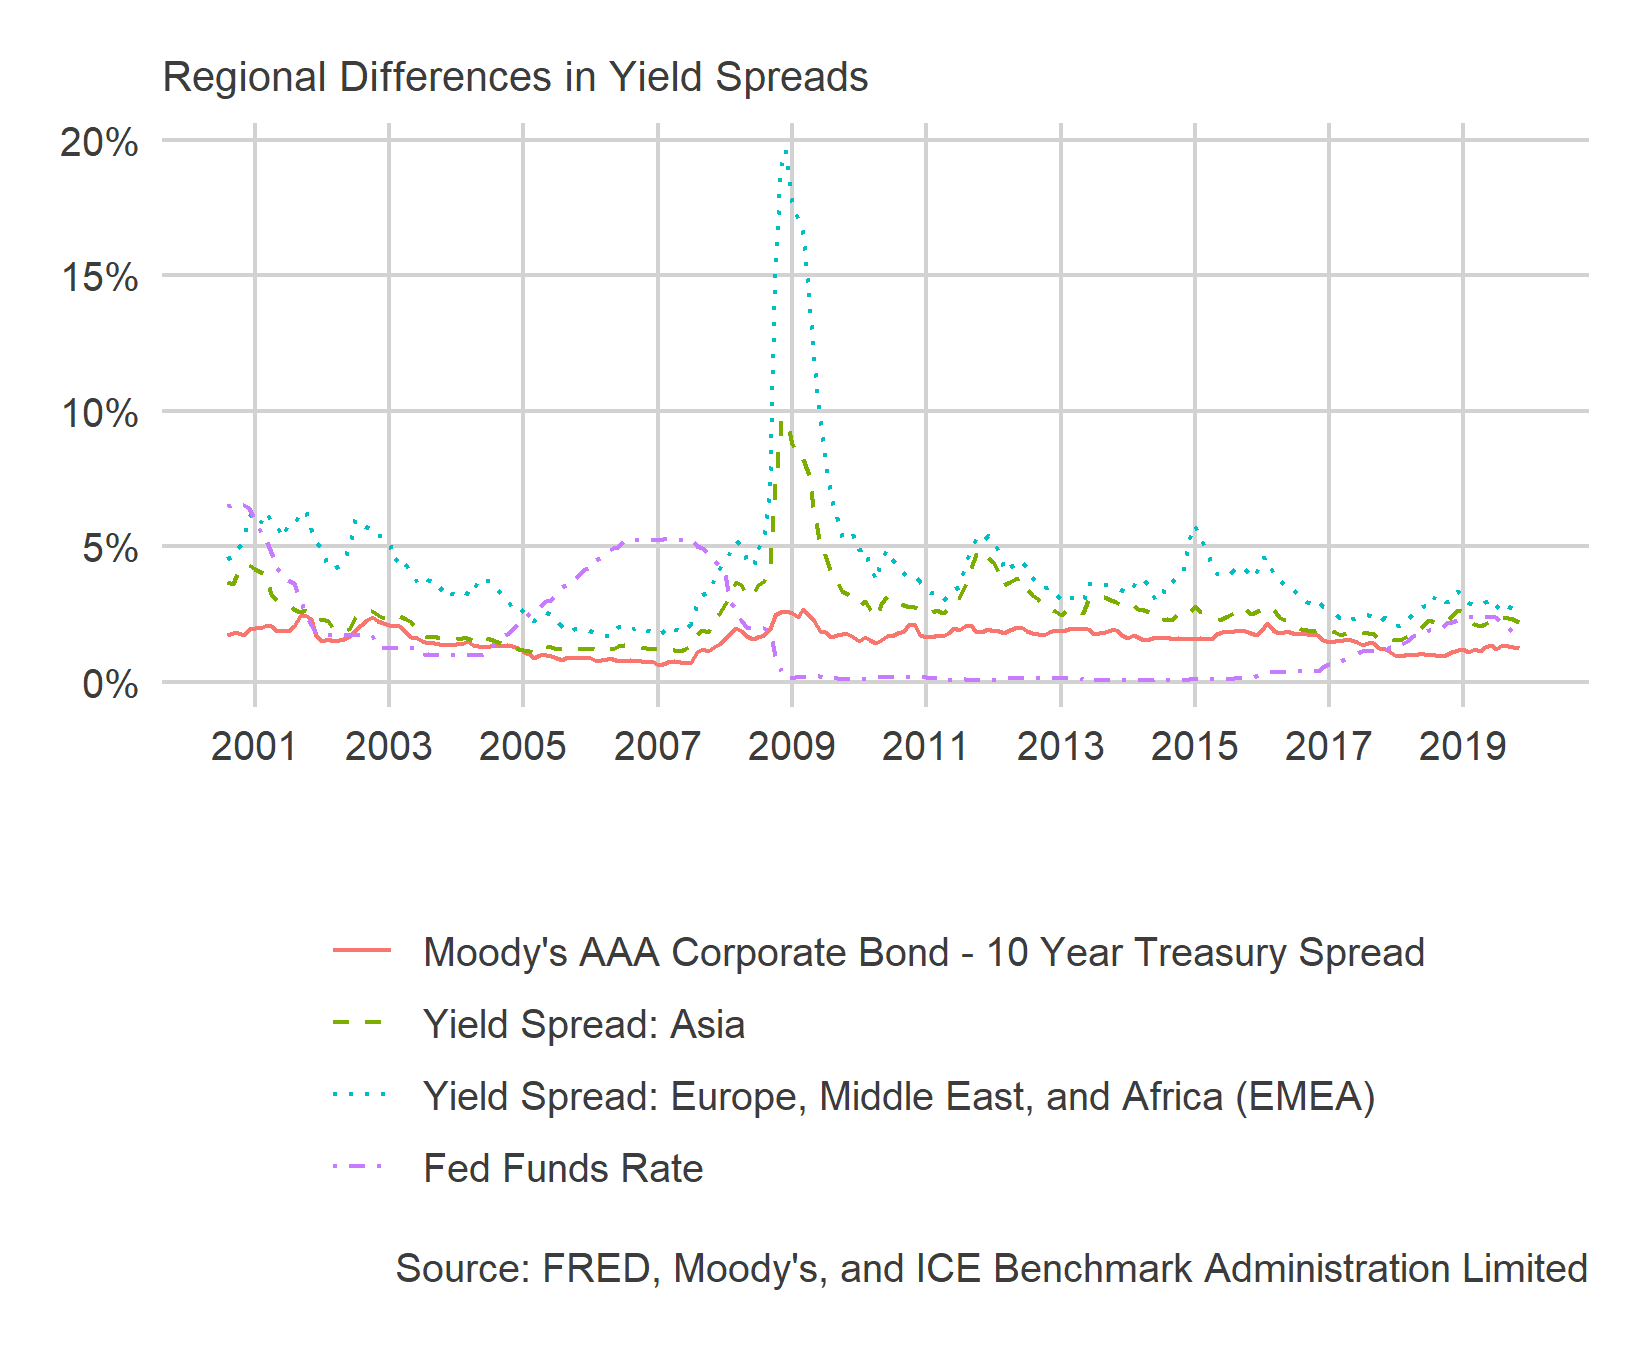
\includegraphics[width=0.8\textwidth]{globalfx.png}
\label{fig:globalfx}
\end{figure}
In this paper, I analyze the relationship between U.S. monetary policy and financing conditions in international markets for emerging market economies, accounting for country-specific factors and changes in the relationship across different time periods.

First, I investigate the effects of the federal funds rate (FFR) on emerging market bond yield spreads with the goal of understanding monetary policy transmission from advanced to emerging economies. I find that changes in the FFR have negative and significant effects on bond spreads. In addition, I find that changes in the FFR have significant but asymmetric effects on sovereign bond spreads in specific EMEs, controlling for country-specific economic conditions, fiscal conditions, exposure to foreign economies, protection against external crises, and global uncertainty. However, the direction of this monetary policy spillover is uncertain, and other country-specific factors could determine both the changes in spreads.

Second, the effects of different time periods are mostly insignificant in the fixed effects model and in individual countries, although the Taper Tantrum was predicted to increase spreads. The primary conclusion from the time-based effects indicate that EMEs still rely on U.S. monetary policy, even in the post-crisis period.

EME central banks struggle with greater exposure to supply shocks and pro-cyclical fiscal policy compared to advanced economies~\parencite{frankel10}. Therefore, studying EME reactions to changes in global economics determinants is critical. Because of cross-country differences between EMEs (in terms of their history, governments, and central banks), there is reason to believe U.S. monetary policy could be transmitted asymmetrically across countries~\parencite{dudley14}. Time and country-based effects could be present and are investigated in this research. 

Although other economists have utilized micro-level banking data~\parencite{buch19} and asset price responses to unconventional monetary policy~\parencite{bowman14}, this research takes a macro-level approach with a panel of long-timeframe data compared with past empirical analyses. Furthermore, the variables used in this research are ``unbundled'' instead of indexed. This paper also disentangles country-based effects with separate regressions for each country in addition to the basic model. These are approaches suggested in the conclusion of~\textcite{comelli12}. Finally, the decoupling debate is lacking for monetary policy transmission, and this paper seeks to provide some evidence towards resolving the decoupling question.

The paper proceeds as follows: Section~\ref{section:background} reviews the relevant literature on monetary policy transmission, Section~\ref{section:data} describes the data, Section~\ref{section:model} estimates the models, Section~\ref{section:results} describes the results of the regression framework, and Section~\ref{section:conclusion} concludes.
%
%
%
%
%
\section{Background}
\label{section:background}
While this project attempts to marry monetary policy transmission with the determinants of sovereign bond spreads, an abundance of literature exists on each of the two separate components. I lay out stylized facts when the literature is in agreement while discussing disagreements when warranted.
\subsection{Monetary Policy Transmission}
U.S. monetary policy vis-a-v\`{i}s the policy rate is undoubtedly a main driver of market decisions. The literature universally uses the FFR as an explanatory or covariate variable for market analyses because of the strength of the correlation between fixed-income securities and the FFR. Although economists debate whether the Fed leads or lags behind the market, shorter-term treasuries closely follow the trajectory of the FFR while longer-term treasuries show a weaker relationship with the interest rate~\parencite{reinhart5}. This predicts an inverse relationship between the FFR and U.S. Treasury Spreads.

In international markets, the effects of U.S. central banking can be divided into two channels. First, central banks often model U.S. central bank design and innovations.~\textcite{balls18} revisit the intuition behind central bank independence, developing guiding principles for modern central banking based on lessons from advanced economies. Many emerging markets are also trending towards open economic models without fixed exchange rate regimes while improving central banking regulatory frameworks in line with the Fed~\parencite{dudley14}.

Second, central bank policy rates and market indicators move with U.S. monetary policy and markets.~\textcite{klemm14} suggest U.S. interest rate changes still precipitate changes in EME bond yields (albeit at a ratio less than one-to-one). These dependencies are especially apparent in times of economic stress, such as the 2013 Taper Tantrum, when the Fed announced its intention to slow Quantitative Easing (QE) programs earlier than expected.~\textcite{Hernandez17} studies the relationship between policy rates in a two-country DSGE model with a foreign country (the United States) and domestic country (the EME). Estimating Bayesian parameters of the model for Mexico indicates that an increase (decrease) in the FFR calls for an increase (decrease) in Mexico's policy rate that is more than one-to-one.~\textcite{rey16} presents evidence that both short-term interest rates and longer-term expectations are transmitted internationally in neo-Keynesian models, even with flexible exchange rate regimes. The primary vehicle for this transmission is the dollar because of its foundational role in global transactions. Finally,~\textcite{chen11} use a global vector error-correcting model to differentiate between the asymmetric effects of QE on advanced economies and EMEs, finding that emerging markets have stronger reactions, with large co-movements in credit growth, capital inflow, currency appreciation, and inflation.
\subsubsection{Decoupling}
The Financial Crisis and Great Recession have called into question ``fundamental'' facts about EME-advanced economy relationships. The literature agrees that EMEs had heterogeneous experiences during the crisis, but the specifics of this experience are hotly debated.~\textcite{llaudes10} employ cross-country empirical analyses, demonstrating that the crisis had greater effects on countries with initially weaker fundamentals and greater linkages to other economies. This differs from previous literature that found no significant link between reserves and downturn.

However, the literature on decoupling, or the disconnect between EME-advanced economy business cycle fluctuations, is mixed.~\textcite{kuzucu17} broadly reviews empirical studies on decoupling, finding that the most convincing papers support decoupling because EMEs demonstrated increased resilience beginning in 2000. Similarly,~\textcite{kose10} conduct fundamental analysis to measure the resilience of EMEs; they find that EMEs were better insulated from crisis and have higher potential for sustained growth.

\textcite{walti12} utilizes both traditional econometric methods and a graphical method to test for independence in business cycles, concluding that no evidence exists for a structural break that would support the decoupling hypothesis. In line with the anti-decoupling camp,~\textcite{takats14} show that the co-movement of long-term U.S. and EME interest rates became stronger after the crisis. Yet another hypothesis is that although real economies are decoupling, financial assets are becoming more synchronized due to stronger financial globalization~\parencite{yeyati12}. 10 years after the end of the Great Recession, monetary policy transmission deserves a closer look.

\subsection{Determinants of EME Bond Spreads}
The literature on sovereign yield spreads determinants is vast but inconclusive given recent global shifts in market stability.\footnote{The literature behind the choices for the model and variables used in this analysis are described in detail in the~\hyperref[section:data]{Data} and~\hyperref[section:model]{Model} sections of this paper.}~\textcite{csonto13} and~\textcite{bellas10} disentangle global and country-specific determinants through component decomposition. They show that global factors are the main determinant of spreads in the short run while country fundamentals are central in the long run.~\textcite{ozmen16} investigate credit ratings, finding that speculative episodes and global indicators are critical for EME spreads. The literature overwhelmingly agrees that EME spreads are shaped not only by country-specific factors but also by global factors that can be proxied by volatility indices, advanced economy bond yields or spreads, and LIBOR rates.
%
%
%
%
%
\section{Data}
\label{section:data}
I use an unbalanced panel dataset of 249 monthly observations between January 1997 and November 2017 for 16 emerging markets in three regions.\footnote{For presentation purposes, the countries are divided into BRICSMINT economies, which consist of Brazil, Russia, China, South Africa, Mexico, and Indonesia and ``other developing economies.'' The exclusion of India was due to the lack of data on Indian sovereign spreads. The exclusion of Nigeria was due to the lack of credit rating data.} The sovereign spread measure was the J.P. Morgan Emerging Markets Bonds Spreads (EMBI+), which was obtained from the World Bank's Global Economic Monitor (GEM) database. The EMBI+ evolved from the Emerging Market Bonds Index (EMBI), adding U.S. dollar local markets instruments, performing loans, Eurobonds, and investment-grade issuers to the original total-return EMBI of U.S. dollar-denominated Brady bonds and other sovereign restructured bonds~\parencite{gaillard12}. The EMBI is widely used by economists to studying EMEs and by market analysts for investment decisions~\parencite{ms19}.

I divide explanatory variables into six categories: (1) U.S. monetary policy, (2) country-specific economic conditions, (3) country-specific fiscal conditions, (4) exposure to foreign economies,  (5) global uncertainty, and (6) time period indicators.
\subsection{U.S. Monetary Policy}
The main explanatory variable that proxies for U.S. monetary policy is the effective federal funds rate (FFR), which is the rate banks charge for overnight interbank loans. This variable was chosen because the frequency of changes is high relative to other tools of the Federal Reserve, such as reserve requirements and the discount rate. The targets for the FFR are based on decisions made by the Federal Open Market Committee, the central policy-setting organization of the United States. The FFR data are from Federal Reserve Economic Database (FRED).
\subsection{Country-specific Economic Conditions}
I include GDP growth and inflation as covariates for a country's economic condition. GDP growth reveals information about a country's propensity to pay back debt in the future. Faster growth helps a country pay debt faster and lowers the probability of default, thus reducing spreads~\parencite{eichengreen00}. GDP growth is constructed from the GEM and is expressed as real year-over-year growth for each quarter and extended across quarters.

Inflation is another measure of macroeconomic stability.~\textcite{cantor96} show that lower inflation is associated with safety and  reduces spreads. Inflation is a major determinant of emerging market risk premia, as~\textcite{aizenman13} discuss in the context of Credit Default Swap spreads. An alternative view is that higher inflation expands the tax base, relaxing a country's debt-financing constraints and increasing its creditworthiness~\parencite{nickel09}. The majority of the literature agrees with the first perspective:  inflation is negatively correlated with spreads~\parencite{eichengreen00}. Inflation data are from the GEM Consumer Price Index (CPI) data, which is expressed as year-over-year percent change in nominal, non-seasonally adjusted consumer prices for a basket of goods.

Additionally, sovereign credit ratings are an institutionally-determined measure for macroeconomic conditions that affect solvency~\parencite{cantor96}.~\textcite{ozmen16} empirically show that credit ratings reflect domestic fundamentals and the participants of rating decisions accurately forecast debt conditions. The sovereign ratings were obtained from~\parencite{emiru19}, which were originally from Bloomberg and the three major rating agencies (Moody's, Standard \& Poor's, and Fitch). The data were transformed using the linear transposition scales in~\parencite{bhatia02}.\footnote{See Table~\ref{tbl6} for the scales.} Higher credit ratings are associated with higher likelihood of default and therefore higher bond spreads.

I use total reserves measured by the months of imports of merchandise goods covered as a proxy for economic resilience in the case of an adverse economic event. Total reserves are a component of the International Country Risk Guide's calculation for financial risk~\parencite{comelli12}. A country's stock of reserves is predicted to have a negative relationship with spreads because a country with a higher quantity of reserves has a smaller risk of defaulting~\parencite{moghadam11}. These data were obtained from the GEM.

Finally, I add a categorical variable for the income condition of the country. These data are from the World Bank Atlas and classify countries as low income, lower middle income, upper middle income, and high income for lending decisions.
\subsection{Country-specific Fiscal Conditions}
Two measures of fiscal conditions are utilized: the central government debt to GDP and the government deficit to GDP ratios. Both are widely accepted in the literature as determinants of credit ratings and bond spreads~\parencite{capelli19,gruber12}. Higher levels of debt and/or deficit indicate a country is less creditworthy and has higher default risk. These fiscal indicators are predicted to have positive effects on bond spreads. The debt to GDP ratio were obtained from the International Monetary Fund's (IMF) Global Debt Database. The deficit to GDP ratios were constructed from the expenditure to GDP and revenue to GDP ratios from the IMF Fiscal Monitor.
\subsection{Exposure to Foreign Economies}
Exchange rates are an unexplored predictor for bond spreads, although~\textcite{edwards86} describes the Real Effective Exchange Rate (REER) as a possible determinant of a country's probability of default. For this research, the REER measures a country's currency competitiveness and signals ``misaligned'' valuations that may lead to currency crises. The REER is measured by the percentage deviation of the REER from its 10-year simple moving average, following~\textcite{jahjah13}, who show that overvalued REERs increase spreads by decreasing debt sustainability. REER is thus predicted to negatively impact bond spreads~\parencite{tebaldi18}. The REER data is downloaded from the GEM.

The traditional measure for openness --- the sum of exports and imports to GDP ratio --- was employed to measure whether high levels of exposure to the global economy were important for bond spreads. Higher openness is predicted to decrease the probability of external default~\parencite{bellas10}, and openness is associated with long-term economic growth~\parencite{ulasan12}. Openness is  predicted to have a negative sign.
\subsection{Global uncertainty}
The Chicago Board Options Exchange Volatility Index (VIX) is closely and positively correlated with EMBI+ spreads and is one of the main global factors that determine bond spreads~\parencite{jaramillo11}. The VIX is a standard proxy for the risk appetite of global investors~\parencite{csonto13}. The data source is FRED.
\subsection{Time Period Indicators}
Indicator variables are constructed for three time periods. The ``recession'' indicator was prepared for the 2001:Q1 to 2001:Q3 recession and the 2007:Q4 to 2009:Q2 recessions. A ``Great Recession'' indicator was prepared for the 2007-09 recession. A ``Taper Tantrum'' indicator was prepared for the period after May 22, 2013, which is when the Federal Reserve announced the possibility of ``tapering'' its fixed income purchases from QE. This tapering resulted in a rise in emerging market bond yields~\parencite{klemm14}.
%
\begin{table}[!htbp]
\scriptsize
\centering
\caption{Descriptive Statistics}
    \label{tbl1}
\begin{tabular}{@{\extracolsep{5pt}}llcc} 
\\[-1.8ex]\hline \hline\\[-1.8ex] 
Variable & Description & Mean (SD) & [Min, Max]\\ 
\hline\\
[-1.8ex] embi & EMBI+ Spread (percentage points) & 3.83 (6.42) & [0.20, 68.6]\\
effr & Federal Funds Rate (percent) & 2.32 (2.31) & [0.04, 6.86]\\
gdp & GDP Growth (percent) & 0.04 (0.04) & [-0.18, 0.15]\\
cpi & CPI Inflation (percent) & 7.52 (11.40) & [-2.45, 126]\\
debt & Debt/GDP Ratio (percent) & 43.2 (22.1) & [4.09, 152]\\
deficit & Deficit/GDP Ratio (percent) & -2.51 (3.14) & [-12.90, 7.91]\\
reer & Real Effective Exchange Rate (percent) & 0.04 (10.60) & [-58.10, 50.60]\\
open & Openness (percent) & 65.60 (41.20) & [16.40, 220.00]\\
rating & Credit Rating & 10.3 (3.43) & [4.33, 22.3]\\
reserves & Months of Import Cover & 9.67 (5.80) & [1.20, 34.40]\\
vix & CBOE Volatility Index & 20.7 (8.11) & [10.4, 62.70]\\
\hline \hline \\[-1.8ex] 
Source:  & \multicolumn{3}{l}{FRED, IMF, Bloomberg, World Bank, and author's calculations} \\ 
\end{tabular} 
\end{table} 

% Table created by stargazer v.5.2.2 by Marek Hlavac, Harvard University. E-mail: hlavac at fas.harvard.edu
% Date and time: Thu, Dec 12, 2019 - 1:34:29 AM
\begin{table}[!htbp] \centering 
  \caption{Pairwise Correlations} 
  \label{tbl2} 
\scriptsize 
	\begin{adjustwidth}{-.5in}{-.5in}
		\begin{center}
			\begin{tabular}{@{\extracolsep{5pt}} cccccccccccc} 
				\\[-1.8ex]\hline 
				\hline \\[-1.8ex] 
				 & spread & gdp & cpi & debt & deficit & exchange & reserve & openness & ratings & VIX & EFFR \\ 
				\hline \\[-1.8ex] 
				spread & $1$ & $$ & $$ & $$ & $$ & $$ & $$ & $$ & $$ & $$ & $$ \\ 
				gdp & $$-$0.210$ & $1$ & $$ & $$ & $$ & $$ & $$ & $$ & $$ & $$ & $$ \\ 
				cpi & $0.420$ & $$-$0.110$ & $1$ & $$ & $$ & $$ & $$ & $$ & $$ & $$ & $$ \\ 
				debt & $0.510$ & $$-$0.180$ & $0.250$ & $1$ & $$ & $$ & $$ & $$ & $$ & $$ & $$ \\ 
				deficit & $0.020$ & $0.370$ & $$-$0.200$ & $$-$0.450$ & $1$ & $$ & $$ & $$ & $$ & $$ & $$ \\ 
				exchange & $$-$0.370$ & $0$ & $$-$0.270$ & $$-$0.230$ & $$-$0.070$ & $1$ & $$ & $$ & $$ & $$ & $$ \\ 
				reserve & $$-$0.020$ & $0.030$ & $$-$0.130$ & $$-$0.260$ & $0.280$ & $0.010$ & $1$ & $$ & $$ & $$ & $$ \\ 
				openness & $$-$0.160$ & $$-$0.020$ & $$-$0.130$ & $0.200$ & $$-$0.040$ & $$-$0.070$ & $$-$0.290$ & $1$ & $$ & $$ & $$ \\ 
				ratings & $0.580$ & $$-$0.140$ & $0.430$ & $0.530$ & $$-$0.130$ & $$-$0.140$ & $$-$0.230$ & $$-$0.340$ & $1$ & $$ & $$ \\ 
				VIX & $0.150$ & $$-$0.230$ & $0.110$ & $$-$0.010$ & $$-$0.070$ & $$-$0.070$ & $0.010$ & $$-$0.030$ & $0.040$ & $1$ & $$ \\ 
				EFFR & $0.070$ & $0.150$ & $0.170$ & $$-$0.030$ & $0.140$ & $0.060$ & $$-$0.190$ & $$-$0.020$ & $0.130$ & $0.010$ & $1$ \\ 
				\hline \\[-1.8ex] 
			\end{tabular} 
		\end{center}
	\end{adjustwidth}
\end{table}
%
%
%
\section{Model}
\label{section:model}
I closely follow~\textcite{edwards86} in constructing the theoretical model for bond pricing and spreads.~\textcite{csonto13} and~\textcite{comelli12} follow the same method. However, I modify the model to account for data with negative values. When there is a non-zero probability of default and investors are price-takers, the equilibrium condition is:
\begin{equation}
\label{eq1}
(1-p(X_{it}))(1+i_{t}+s_{it}) = (1+i_{t})
\end{equation}
 for a one-period bond, where $i_{t}$ is the global risk-free interest rate at time $t$, $p(X_{it})$ is the probability of default based on country fundamentals of $X_{it}$, and $s_{it}$ is the country's risk premium. We rearrange (\ref{eq1}) to isolate $s_{it}$.
 \begin{equation}
 \label{eq2}
 s_{it} = \dfrac{(1+i_{t})}{(1-p(X_{it}))}-(1+i_{t}) = (1+i_{t})\dfrac{p(X_{it})}{1-p(X_{it})}
 \end{equation}
 Per~\textcite{edwards86}, the probability of default has the logistic form
\begin{equation}
\label{eq3}
p(X_{it}) = \dfrac{exp(\Sigma \beta_{i}X_{it})}{1+exp(\Sigma \beta_{i}X_{it})}
\end{equation}
where $\beta_{i}$ are the coefficients that determine the probability of default. Substituting into the right-hand side of~\ref{eq2}, the country risk premium (i.e. bond spread) becomes
\begin{equation}
\label{eq4}
 s_{it} = (exp \Sigma \beta_{i}X_{it})(1+i_{t})
\end{equation}
with the logarithmic form of 
\begin{equation}
\label{eq5}
 ln(s_{it}) = ln(\Sigma \beta_{i}X_{it}) + ln(1+i_{t}) + \varepsilon_{it} 
\end{equation}
with the added error term of $\varepsilon_{it}$.

For the regression framework, I modify (\ref{eq5}) to account for the possibility of negative data that haved undefined natural logarithms. I use the following specification for the fixed effects estimation:
\begin{multline}
\label{eqn6}
ln(embi_{it}) = \alpha_{1}ln(effr_{t}) + \beta_{1}gdp_{it} + \beta_{2}cpi_{it} + \beta_{3}debt_{it} + \beta_{4}deficit_{it} + \beta_{5}reer_{it}\\ + \beta_{6}open_{it} + \beta_{7}rating_{it} + \beta_{8}ln(reserves_{it}) + \alpha_{2}ln(vix_{t}) + \gamma_{(1,3)}time + \mu_{i} + \varepsilon_{it}
\end{multline}
where the coefficients for global factors, country-specific factors, time factors, and the country fixed effect are $\alpha$, $\beta$, $\gamma$, and $\mu$, respectively. This follows the modelling procedure from~\textcite{capelli19}. The Hausman test (not reported) strongly rejects the random effects model, so the fixed effects model is employed.
%
%
%
% 
\section{Results}
\label{section:results}
\subsection{Fixed Effects Model on Whole Sample}
First, I estimate equation (\ref{eqn6}) on the whole sample. The explanatory variables vary across each specification, but the results indicate that both country-specific factors and global factors are determinants of bond yield spreads (Table~\ref{tbl3}) while the FFR is a significant explanatory variable in all but one specification.
% Table created by stargazer v.5.2.2 by Marek Hlavac, Harvard University. E-mail: hlavac at fas.harvard.edu
% Date and time: Tue, Dec 10, 2019 - 12:56:24 AM
\begin{table}[!htbp] \centering 
  \caption{Fixed Effects Estimation of Sovereign Bond Spreads} 
  \label{tbl3} 
\scriptsize
\begin{tabular}{@{\extracolsep{5pt}}lcccc} 
\\[-1.8ex]\hline 
\hline \\[-1.8ex] 
 & \multicolumn{4}{c}{\textit{Dependent variable:}} \\ 
\cline{2-5} 
\\[-1.8ex] & \multicolumn{4}{c}{log(EMBI+ Spreads)} \\ 
\\[-1.8ex] & (1) & (2) & (3) & (4)\\ 
\hline \\[-1.8ex] 
 log(EFFR) & $-$0.028$^{***}$ & $-$0.130$^{***}$ & $-$0.053 & $-$0.107$^{***}$ \\ 
  & (0.006) & (0.023) & (0.201) & (0.021) \\ 
  GDP Growth & $-$3.163$^{***}$ & $-$2.997$^{***}$ & $-$0.536 & $-$3.458$^{***}$ \\ 
  & (0.267) & (0.274) & (0.447) & (0.313) \\ 
  CPI Inflation & 0.005$^{***}$ & 0.006$^{***}$ & 0.013$^{***}$ & $-$0.007$^{***}$ \\ 
  & (0.001) & (0.001) & (0.001) & (0.003) \\ 
  Debt to GDP Ratio & 0.011$^{***}$ & 0.011$^{***}$ & 0.001 & 0.015$^{***}$ \\ 
  & (0.001) & (0.001) & (0.001) & (0.001) \\ 
  Deficit to GDP Ratio & $-$0.004 & $-$0.005 & $-$0.021$^{***}$ & $-$0.004 \\ 
  & (0.004) & (0.004) & (0.007) & (0.005) \\ 
  REER & $-$0.008$^{***}$ & $-$0.008$^{***}$ & $-$0.014$^{***}$ & $-$0.004$^{***}$ \\ 
  & (0.001) & (0.001) & (0.001) & (0.001) \\ 
  Openness & 0.002$^{***}$ & 0.002$^{**}$ & $-$0.005$^{**}$ & 0.001$^{*}$ \\ 
  & (0.001) & (0.001) & (0.002) & (0.001) \\ 
  Credit Rating & 0.091$^{***}$ & 0.092$^{***}$ & 0.059$^{***}$ & 0.115$^{***}$ \\ 
  & (0.006) & (0.006) & (0.013) & (0.006) \\ 
  log(Reserves) & $-$0.102$^{***}$ & $-$0.111$^{***}$ & $-$0.542$^{***}$ & 0.028 \\ 
  & (0.022) & (0.022) & (0.041) & (0.025) \\ 
  log(VIX) & 0.620$^{***}$ & 0.636$^{***}$ & 0.494$^{***}$ & 0.636$^{***}$ \\ 
  & (0.027) & (0.027) & (0.048) & (0.030) \\ 
  Recession Dummy & 0.189$^{***}$ & $-$0.239 & $-$0.118 & $-$0.259 \\ 
  & (0.043) & (0.364) & (0.568) & (0.407) \\ 
  Great Recession Dummy & $-$0.236$^{***}$ & 0.191 & 0.240 & 0.242 \\ 
  & (0.048) & (0.365) & (0.569) & (0.408) \\ 
  Taper Dummy & 0.146$^{***}$ & 0.225$^{***}$ & 0.852$^{***}$ & 0.087$^{**}$ \\ 
  & (0.022) & (0.039) & (0.074) & (0.042) \\ 
  Lower Middle Income Dummy &  & $-$0.047 & $-$0.203 & 0.140$^{*}$ \\ 
  &  & (0.062) & (0.474) & (0.072) \\ 
  Upper Middle Income Dummy &  & 0.035 & $-$0.067 & $-$0.011 \\ 
  &  & (0.050) & (0.472) & (0.047) \\ 
  Lower Income Dummy &  & $-$3.648$^{***}$ & $-$2.819$^{***}$ &  \\ 
  &  & (0.463) & (0.664) &  \\ 
  log(EFFR)*Recession &  & 0.290 & 0.199 & 0.298 \\ 
  &  & (0.237) & (0.369) & (0.265) \\ 
  log(EFFR)*Great Recession &  & $-$0.301 & $-$0.263 & $-$0.311 \\ 
  &  & (0.238) & (0.369) & (0.265) \\ 
  log(EFFR)*Taper &  & 0.058$^{***}$ & 0.219$^{***}$ & 0.051$^{**}$ \\ 
  &  & (0.019) & (0.033) & (0.020) \\ 
  log(EFFR)*Lower Middle Income &  & 0.101$^{***}$ & $-$0.008 & 0.159$^{***}$ \\ 
  &  & (0.025) & (0.202) & (0.023) \\ 
  log(EFFR)*Upper Middle Income &  & 0.117$^{***}$ & 0.014 & 0.070$^{***}$ \\ 
  &  & (0.023) & (0.201) & (0.021) \\ 
  log(EFFR)*Lower Income &  & 2.366$^{***}$ & 1.726$^{***}$ &  \\ 
  &  & (0.278) & (0.344) &  \\ 
 \hline \\[-1.8ex] 
Observations & 3,306 & 3,306 & 1,341 & 1,965 \\ 
R$^{2}$ & 0.542 & 0.560 & 0.605 & 0.656 \\ 
Adjusted R$^{2}$ & 0.539 & 0.555 & 0.597 & 0.651 \\ 
\hline 
\hline \\[-1.8ex] 
\textit{Note:}  & \multicolumn{4}{l}{$^{*}$p$<$0.1; $^{**}$p$<$0.05; $^{***}$p$<$0.01} \\ 
\multicolumn{5}{l}{Specification (2) is specification (1) with interaction effects. Specification (3) and (4) are}\\
\multicolumn{5}{l}{specification (2) broken into BRICSMINT countries and other EMEs, respectively.}\\
\multicolumn{5}{l}{Standard errors are in parentheses. \textit{Source:} author's calculations.}\\
\end{tabular} 
\end{table} 
As expected, country-specific determinants are important. The variables that proxied for a country's economic health and lending condition were statistically significant across nearly each specification. The magnitude of the coefficient for GDP growth suggests that bond spreads are most sensitive to changes in domestic GDP growth: a 1 percentage point change in GDP growth is associated with a 3.2 percent decrease in the bond spread. CPI inflation is associated with a small but significant positive effect on bond spreads. These results suggest that investors pay close attention to a country's economic indicators. The faster the country is growing and the lower inflation is, the higher the yield on shorter-term sovereign bonds and the lower the spread.

The classic proxy for fiscal condition, the debt to GDP ratio, had a positive coefficient across each specification. However, the coefficient for the less-tested deficit to GDP ratio variable was negative across all specifications. This contradicts conventional wisdom about investor perception of credit risk as a determinant of bond spread. The deficit to GDP ratio could be an insufficient proxy for a country's debt condition because the variable only measures one-year fiscal changes. The statistical significance of the debt to GDP ratio variable suggests that default risk still strongly determines investments. Across all specifications, the credit rating variable was positive, and in the baseline model, a 1 point increase in the rating score was predicted with a 0.091 percentage point increase in bond spreads. As a country changed from one credit rating to another (for example, shifting from Aaa to AA1 in the Moody's system), investors perceived this change as an indication of weakness and decreased creditworthiness.

The negative coefficient on the REER variable suggests that currency overvaluations demonstrate safety or economic strength to investors, who may prioritize short-term investment gains. This is contrary to~\textcite{jahjah13}, who report a positive correlation between spreads and REER overvaluation. Investor patterns may have shifted in the post-crisis era as economic conditions have consistently improved since the Great Recession. The consistent negative and significant value of the coefficient suggest that currency overvaluations and bond spreads should be an area of further study.

The negative value and significance of the coefficient for reserves expressed as total months of goods import cover could be explained by the variable's indication that a country has less vulnerability to external shocks and higher stability. On the other hand, the positive value for openness indicates that increased trade with other countries decreases investment safety. This could be explained by investor perception that countries that must find avenues for international trade instead of domestic production are economically weaker. The results also demonstrate that increases in global risk, as measured by the VIX variable, increase spreads. The VIX coefficient is positive across each specification; a 1 percent increase in the VIX is associated with a 0.49-0.64 percent increase in spreads. This suggests global volatility is a key explanatory variable for investor decisions for EME bonds.

The FFR can be thought of as a proxy for global risk aversion via liquidity conditions, per~\textcite{csonto13}. The coefficient on the FFR is negative and significant for all but BRICS and MINT EMEs. In the baseline model, a 1 percent change in the FFR is associated with a 0.028 percentage point decrease in EME Spreads. The U.S. policy rate is negatively correlated with global volatility --- as economic conditions grow more dire, the Fed often responds or leads with FFR cuts. The asymmetric magnitude and significance of the effective FFR variable across BRICSMINT and other EMEs motivated a closer analysis of individual countries and different groups of countries (see Table~\ref{tbl4} and Table~\ref{tbl5}).

The negative value of this coefficient matches recent literature on the topic, but contradicts earlier studies, such as~\textcite{arora01}, which predicted a positive coefficient. In the context of greater economic volatility in the early 21\textsuperscript{st} century, the negative coefficient could be explained by the U.S. position as a safe haven. Although a lower FFR would indicate the possibility of economic weakness in the United States and theoretically drive capital elsewhere, an investor could find market conditions in other countries to be \textit{even riskier} and continue to invest (or increase investment) in U.S. Treasury bonds and securities.
\begin{figure}[h!]
	\caption{Eras of U.S. Central Banking Spillover}
	\centering
	\makebox[\textwidth][c]{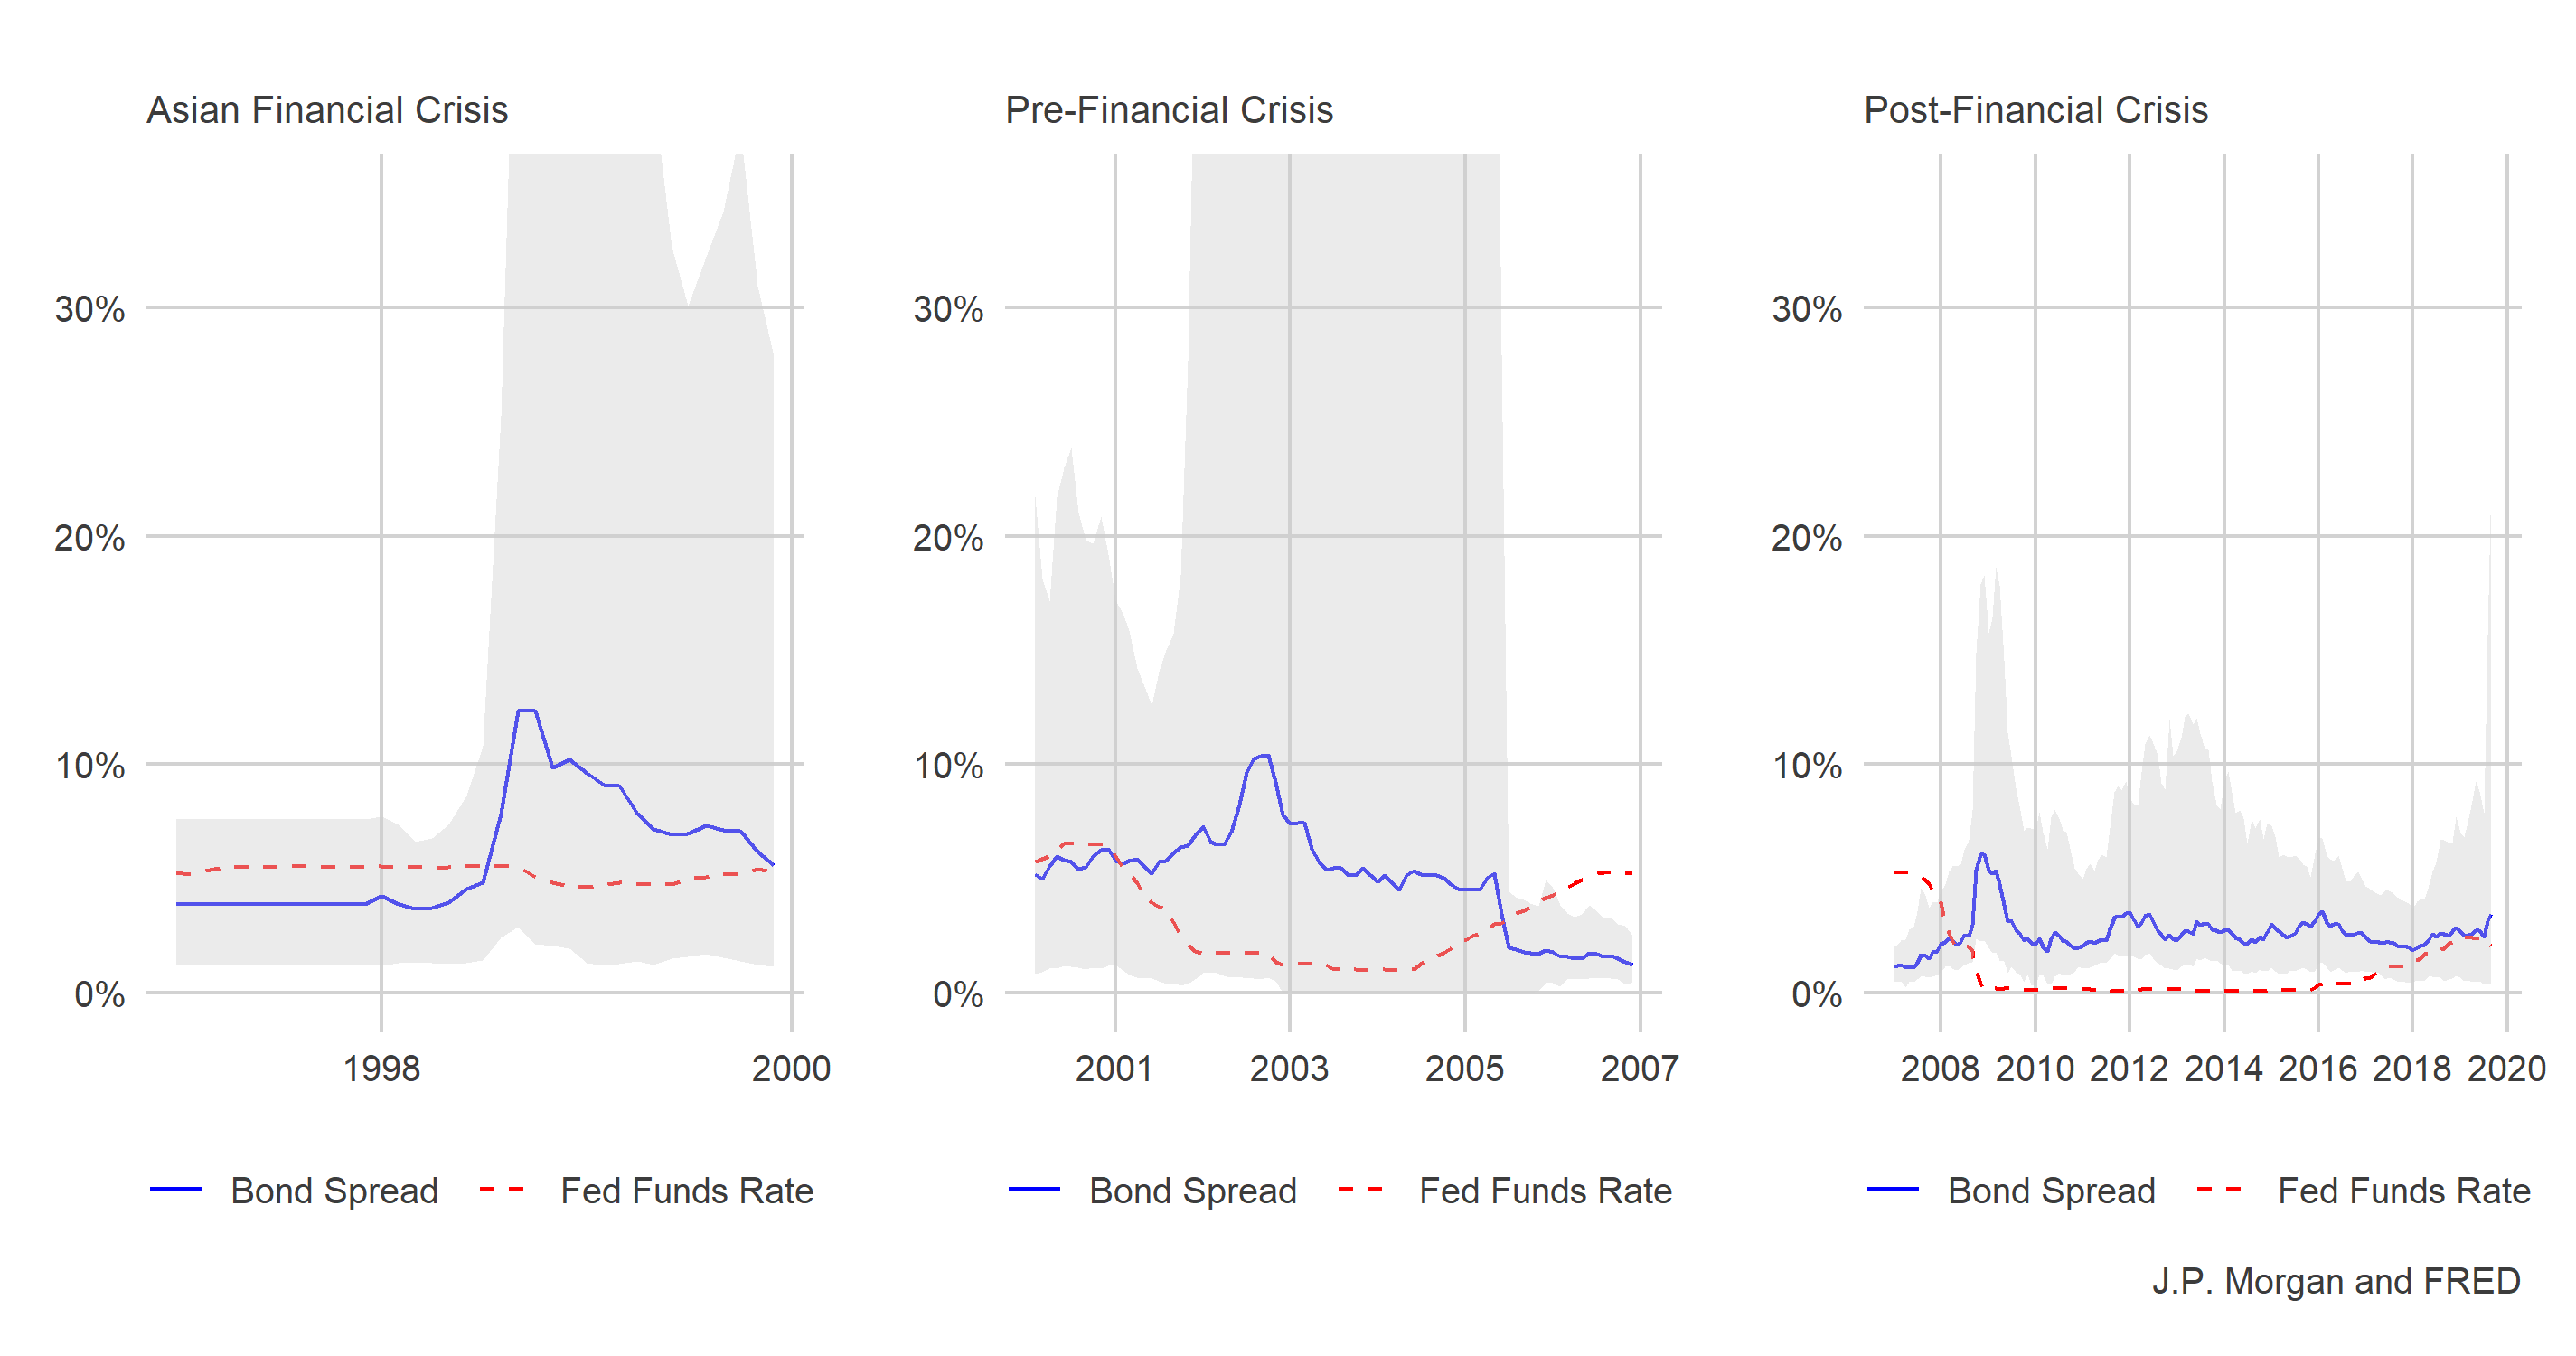
\includegraphics[width=1.1\textwidth]{time.png}}%
	\label{fig:time}
\end{figure}

The results suggested by the time dummies are not entirely clear, although a first-pass analysis shows decreasing variability after 2006 and a negative relationship between the FFR and spreads until approximately 2018. The recession dummy demonstrates a positive association with the bond spread for the baseline regression but a negative association for the other specifications. In times of U.S. crisis, EME bond spreads rise. However, this intuition contradicts the idea of the FFR as a proxy for global liquidity. The safe haven effect may have evolved significantly in the last decade, and the presence of only two recessions makes prescriptive claims on the evolution of the FFR difficult. The negative coefficient for the Great Recession dummy begs the question of whether the effects on bond spreads vary based on the length or severity of a recession. But the positive but statistically insignificant coefficient for this dummy for the other specifications create doubt that there is a consistent effect. The positive coefficient for the Taper Dummy for regressions suggests that the Taper Tantrum increased bond spreads. The Fed's decision to dampen QE could have scared investors planning on the Fed's purchase of securities to appreciate bond yields, injecting higher volatility in the fixed income market and driving spread increases. This is supported by the positive and significant coefficient on the interaction variable for the FFR and the Taper Tantrum dummy. During the Taper Tantrum, increases in the FFR were predicted to further increase bond spreads.

The income variables also lack clear interpretations, due to high variability. The interaction of the FFR and income variables, while significant, yield questionable interpretations about the effect of different incomes on monetary policy transmission. The insignificance of the majority of income-related coefficients questions whether a quantitative income variable should be used instead of a categorical classifier.

The chosen variables for bond determinants explain spreads reasonably well, with adjusted $R^{2}$ value between 0.54 and 0.65 dependent on the specification.
%
%
%
%
\subsection{Specific Country Regressions}
Second, I estimate equation (\ref{eqn6}) without the fixed effects coefficient by using individual country data. The regressions are  calculated individually for each of the countries in the panel.\footnote{The income variable and interaction effects with the income variable are removed in the specific country regressions because of the lack of different levels. Certain countries only reported one income level throughout the sample period, making the regression impossible to compute with a high degree of multicollinearity.}

By and large, the covariates for individual countries had the same sign and similar magnitude to the coefficient in the fixed effects model in Table~\ref{tbl3} with more variability. The coefficient for GDP growth is negative, large, and statistically significant across nearly every country. The coefficients for the time indicators and their interactions with the FFR are indiscernible, with no clear patterns or directions. This lends credence to the lack of decoupling business cycles between EMEs and advanced economies in terms of monetary policy transmission, as the Great Recession and the Taper Tantrum have had insignificant effects on spreads. If EMEs had greater insulation from the financial crisis and other global factors, the coefficients for recessionary or volatility-based dummies would be expected to be negative.

The coefficient for debt to GDP Ratio had greater variation across countries both in terms of sign and magnitude when compared to the fixed effects model. Countries could be borrowing at high levels to complete internal projects that are key to stability; countries could also be borrowing to invigorate the economy amidst a downturn. The variety of reasons for higher debt ratios based on incomplete investor information complicates the explanation of variables for individual countries. Interestingly, the REER variable consistently displayed negative significant effects, supporting the hypothesis that overvaluations depress spreads.

The FFR has significant effects as a predictor across 10 of the 16 countries in the panel. Five of these coefficients are negative, and the rest are positive. The FFR coefficient displays a negative sign in the fixed effects regression, demonstrating the biasing effects of sample size weights that should be disentangled in individual country regressions. Countries that have a positive FFR coefficient may have a ``normal'' relationship with U.S. economic conditions. In other words, a rising FFR can signal a healthier U.S. economy (although with higher inflation risk) in comparison to EMEs. That encourages investors to buy U.S. securities and drives up the risk premia that investors require for EME assets to match the safety of the U.S. market. The opposite effect would hold true for a falling FFR, which indicates a weaker economy. Safe haven theory indicates that the inherent structure of the U.S. market makes the United States safer in critical periods. The asymmetry of the FFR coefficient across countries and different time periods leaves room for further empirical work that could use event-study methods for individual countries. U.S. monetary policy via the FFR still affects EME markets; however, the mechanism by which such transmission occurs is uncertain.

The positive sign and significance across nearly every country for the VIX variable shows the strength of the VIX in predicting global economic uncertainty. The consistency of the coefficient suggests that global factors still have a critical influence on bond-buying decisions for investors.

Overall, the variables predicted movements in country sovereign bond spreads accurately, with a $R^{2}$ value between 0.79 and 0.97 dependent on the country. For the international fixed income market, global variables such as VIX and the FFR still play significant roles in determining the change in spreads across the sample of 16 countries.
%
\begin{landscape}
% Table created by stargazer v.5.2.2 by Marek Hlavac, Harvard University. E-mail: hlavac at fas.harvard.edu
% Date and time: Thu, Dec 12, 2019 - 1:38:56 AM
\begin{table}[!htbp] \centering 
  \caption{Sovereign Bond Spreads of BRICS and MINT Economies with Interactions} 
  \label{tbl4} 
\scriptsize 
\begin{tabular}{@{\extracolsep{5pt}}lccccccc} 
\\[-1.8ex]\hline 
\hline \\[-1.8ex] 
 & \multicolumn{7}{c}{\textit{Dependent variable:}} \\ 
\cline{2-8} 
\\[-1.8ex] & \multicolumn{7}{c}{log(EMBI+ Spreads), by Country} \\ 
 & Brazil & Russia & China & South Africa & Mexico & Indonesia & Turkey \\ 
\\[-1.8ex] & (1) & (2) & (3) & (4) & (5) & (6) & (7)\\ 
\hline \\[-1.8ex] 
 log(EFFR) & $-$0.117$^{***}$ & $-$0.133$^{***}$ & 0.073$^{**}$ & 0.004 & 0.025 & 0.364$^{***}$ & $-$0.023 \\ 
  & (0.022) & (0.017) & (0.032) & (0.025) & (0.018) & (0.071) & (0.019) \\ 
  GDP Growth & $-$3.224$^{***}$ & $-$2.035$^{***}$ & $-$11.132$^{***}$ & $-$2.644$^{**}$ & $-$4.323$^{***}$ & $-$2.427 & 1.137$^{***}$ \\ 
  & (0.645) & (0.483) & (1.429) & (1.173) & (0.529) & (6.561) & (0.389) \\ 
  CPI Inflation & $-$0.013$^{*}$ & 0.003$^{***}$ & 0.029$^{***}$ & $-$0.006 & 0.005 & 0.031$^{*}$ & 0.008$^{***}$ \\ 
  & (0.007) & (0.001) & (0.010) & (0.005) & (0.005) & (0.017) & (0.002) \\ 
  Debt to GDP Ratio & $-$0.005 & 0.026$^{***}$ & $-$0.057$^{***}$ & 0.037$^{***}$ & 0.025$^{***}$ & $-$0.035$^{**}$ & 0.001 \\ 
  & (0.004) & (0.004) & (0.012) & (0.004) & (0.009) & (0.016) & (0.003) \\ 
  Deficit to GDP Ratio & $-$0.083$^{***}$ & 0.030$^{***}$ & $-$0.073$^{**}$ & $-$0.044$^{**}$ & 0.011 & 0.547$^{***}$ & $-$0.024$^{*}$ \\ 
  & (0.015) & (0.007) & (0.028) & (0.019) & (0.018) & (0.130) & (0.013) \\ 
  REER & $-$0.015$^{***}$ & $-$0.015$^{***}$ & 0.004 & $-$0.007$^{***}$ & $-$0.002 & $-$0.077$^{***}$ & $-$0.014$^{***}$ \\ 
  & (0.002) & (0.002) & (0.005) & (0.002) & (0.002) & (0.011) & (0.003) \\ 
  Openness & $-$0.019$^{*}$ & $-$0.039$^{***}$ & $-$0.015$^{***}$ & 0.010$^{**}$ & 0.009$^{***}$ & $-$0.067$^{***}$ & $-$0.007 \\ 
  & (0.010) & (0.007) & (0.003) & (0.005) & (0.003) & (0.023) & (0.007) \\ 
  Credit Rating & 0.176$^{***}$ & 0.092$^{***}$ & $-$0.559$^{***}$ & 0.124$^{***}$ & 0.311$^{***}$ & $-$0.275$^{**}$ & 0.101$^{***}$ \\ 
  & (0.019) & (0.019) & (0.046) & (0.032) & (0.025) & (0.110) & (0.031) \\ 
  log(Reserves) & $-$0.617$^{***}$ & $-$0.236$^{**}$ & $-$0.347$^{***}$ & $-$0.030 & $-$0.024 & $-$1.257$^{***}$ & 0.034 \\ 
  & (0.079) & (0.091) & (0.114) & (0.040) & (0.066) & (0.383) & (0.076) \\ 
  log(VIX) & 0.654$^{***}$ & 0.541$^{***}$ & 0.319$^{***}$ & 0.600$^{***}$ & 0.610$^{***}$ & $-$0.094 & 0.312$^{***}$ \\ 
  & (0.056) & (0.052) & (0.062) & (0.045) & (0.043) & (0.176) & (0.061) \\ 
  Recession Dummy & 0.638 & $-$0.216 & $-$0.047 & $-$0.970$^{**}$ & $-$0.701$^{*}$ & $-$0.583$^{***}$ & $-$1.202$^{*}$ \\ 
  & (0.577) & (0.531) & (0.617) & (0.420) & (0.421) & (0.207) & (0.627) \\ 
  Great Recession Dummy & $-$0.635 & 0.626 & $-$0.055 & 1.392$^{***}$ & 0.748$^{*}$ &  & 1.403$^{**}$ \\ 
  & (0.578) & (0.533) & (0.620) & (0.423) & (0.425) &  & (0.636) \\ 
  Taper Dummy & 0.107 & $-$0.598$^{***}$ & $-$0.193 & $-$0.204$^{*}$ & 0.526$^{***}$ & $-$0.314 & 0.356$^{***}$ \\ 
  & (0.193) & (0.165) & (0.207) & (0.104) & (0.133) & (0.412) & (0.131) \\ 
  log(EFFR)*Recession & $-$0.358 & 0.179 & 0.079 & 0.643$^{**}$ & 0.467$^{*}$ & $-$0.329$^{***}$ & 1.012$^{**}$ \\ 
  & (0.375) & (0.344) & (0.403) & (0.273) & (0.272) & (0.110) & (0.413) \\ 
  log(EFFR)*Great Recession & 0.558 & $-$0.244 & $-$0.047 & $-$0.676$^{**}$ & $-$0.506$^{*}$ &  & $-$1.082$^{***}$ \\ 
  & (0.374) & (0.345) & (0.403) & (0.273) & (0.273) &  & (0.410) \\ 
  log(EFFR)*Taper & 0.113 & $-$0.254$^{***}$ & $-$0.095 & 0.019 & 0.058 & $-$0.091 & 0.035 \\ 
  & (0.078) & (0.069) & (0.069) & (0.043) & (0.047) & (0.139) & (0.051) \\ 
  Constant & $-$0.499 & 0.682 & 6.799$^{***}$ & $-$4.112$^{***}$ & $-$4.883$^{***}$ & 12.506$^{***}$ & $-$1.104$^{*}$ \\ 
  & (0.489) & (0.453) & (0.680) & (0.404) & (0.355) & (2.294) & (0.563) \\ 
 \hline \\[-1.8ex] 
Observations & 232 & 220 & 249 & 202 & 249 & 178 & 213 \\ 
R$^{2}$ & 0.932 & 0.971 & 0.832 & 0.930 & 0.916 & 0.803 & 0.867 \\ 
Adjusted R$^{2}$ & 0.926 & 0.969 & 0.820 & 0.924 & 0.910 & 0.786 & 0.856 \\ 
\hline 
\hline \\[-1.8ex] 
\textit{Note:}  & \multicolumn{7}{l}{$^{*}$p$<$0.1; $^{**}$p$<$0.05; $^{***}$p$<$0.01} \\ 
 & \multicolumn{7}{l}{Standard errors are in parentheses.} \\
 \textit{Source:}  & \multicolumn{7}{l}{author's calculations.} \\  
\end{tabular} 
\end{table} 
\newpage
% Table created by stargazer v.5.2.2 by Marek Hlavac, Harvard University. E-mail: hlavac at fas.harvard.edu
% Date and time: Tue, Dec 10, 2019 - 1:04:42 AM
\begin{table}[!htbp] \centering 
  \caption{Sovereign Bond Spreads of Other Emerging/Developing Market Economies with Interactions} 
  \label{tbl5} 
\scriptsize 
\begin{tabular}{@{\extracolsep{5pt}}lccccccccc} 
\\[-1.8ex]\hline 
\hline \\[-1.8ex] 
 & \multicolumn{9}{c}{\textit{Dependent variable:}} \\ 
\cline{2-10} 
\\[-1.8ex] & \multicolumn{9}{c}{log(EMBI+ Spreads), by Country} \\ 
 & Argentina & Chile & Colombia & Egypt & Hungary & Malaysia & Peru & Philippines & Poland \\ 
\\[-1.8ex] & (1) & (2) & (3) & (4) & (5) & (6) & (7) & (8) & (9)\\ 
\hline \\[-1.8ex] 
 log(EFFR) & $-$0.235$^{***}$ & 0.090$^{***}$ & $-$0.016 & 0.263$^{***}$ & 0.068$^{**}$ & $-$0.076$^{*}$ & $-$0.133$^{***}$ & $-$0.025 & $-$0.252$^{***}$ \\ 
  & (0.029) & (0.024) & (0.018) & (0.069) & (0.034) & (0.040) & (0.045) & (0.020) & (0.029) \\ 
  GDP Growth & $-$2.647$^{***}$ & $-$0.589 & $-$0.811 & $-$4.143$^{***}$ & $-$0.765 & $-$2.914$^{***}$ & $-$0.375 & $-$1.357$^{**}$ & $-$2.608$^{**}$ \\ 
  & (0.616) & (0.571) & (0.676) & (1.552) & (1.102) & (0.919) & (0.626) & (0.648) & (1.147) \\ 
  CPI Inflation & $-$0.030$^{**}$ & 0.047$^{***}$ & 0.021$^{**}$ & 0.027$^{**}$ & 0.019 & $-$0.00004 & 0.058$^{***}$ & 0.052$^{***}$ & 0.053$^{***}$ \\ 
  & (0.013) & (0.009) & (0.010) & (0.012) & (0.013) & (0.011) & (0.016) & (0.007) & (0.009) \\ 
  Debt to GDP Ratio & 0.025$^{***}$ & 0.023$^{***}$ & 0.094$^{***}$ & $-$0.020 & 0.037$^{***}$ & $-$0.013 & 0.008 & 0.006$^{*}$ & $-$0.011 \\ 
  & (0.002) & (0.007) & (0.006) & (0.012) & (0.009) & (0.013) & (0.015) & (0.004) & (0.010) \\ 
  Deficit to GDP Ratio & 0.125$^{***}$ & $-$0.009 & 0.152$^{***}$ & $-$0.161$^{***}$ & $-$0.066$^{***}$ & 0.104$^{***}$ & $-$0.013 & $-$0.058$^{***}$ & 0.097$^{***}$ \\ 
  & (0.041) & (0.009) & (0.015) & (0.048) & (0.018) & (0.028) & (0.034) & (0.012) & (0.016) \\ 
  REER & 0.001 & $-$0.011$^{***}$ & $-$0.011$^{***}$ & $-$0.006 & $-$0.023$^{***}$ & $-$0.038$^{***}$ & $-$0.020$^{***}$ & $-$0.005$^{**}$ & 0.010$^{***}$ \\ 
  & (0.003) & (0.002) & (0.002) & (0.004) & (0.005) & (0.005) & (0.005) & (0.002) & (0.003) \\ 
  Openness & $-$0.065$^{***}$ & $-$0.026$^{***}$ & $-$0.063$^{***}$ & $-$0.034$^{***}$ & 0.007$^{***}$ & $-$0.012$^{***}$ & $-$0.013 & 0.019$^{***}$ & $-$0.005 \\ 
  & (0.014) & (0.005) & (0.009) & (0.012) & (0.002) & (0.003) & (0.012) & (0.003) & (0.005) \\ 
  Credit Rating & 0.080$^{***}$ & $-$0.276$^{***}$ & 0.095$^{**}$ & 0.109$^{*}$ & 0.353$^{***}$ &  & $-$0.038 & $-$0.054$^{***}$ & 0.160$^{***}$ \\ 
  & (0.020) & (0.033) & (0.038) & (0.061) & (0.031) &  & (0.039) & (0.015) & (0.052) \\ 
  log(Reserves) & $-$0.429$^{***}$ & 0.068 & 0.118$^{**}$ & $-$0.418$^{***}$ & 0.347$^{***}$ & $-$0.582$^{***}$ & 0.132 & 0.099 & 0.110 \\ 
  & (0.155) & (0.078) & (0.060) & (0.141) & (0.111) & (0.158) & (0.091) & (0.071) & (0.079) \\ 
  log(VIX) & 0.583$^{***}$ & 0.574$^{***}$ & 0.562$^{***}$ & 0.832$^{***}$ & 0.418$^{***}$ & 0.495$^{***}$ & 0.622$^{***}$ & 0.398$^{***}$ & 0.912$^{***}$ \\ 
  & (0.107) & (0.042) & (0.045) & (0.150) & (0.072) & (0.063) & (0.059) & (0.045) & (0.063) \\ 
  Recession Dummy & 1.065 & $-$0.060 & 0.046 & 0.416$^{***}$ & $-$2.015$^{**}$ & 0.285$^{***}$ & 0.267$^{**}$ & 0.028 & $-$0.072 \\ 
  & (1.159) & (0.392) & (0.379) & (0.145) & (0.785) & (0.077) & (0.111) & (0.425) & (0.648) \\ 
  Great Recession Dummy & $-$0.958 & 0.314 & 0.044 &  & 2.546$^{***}$ &  &  & 0.131 & $-$0.060 \\ 
  & (1.162) & (0.397) & (0.380) &  & (0.791) &  &  & (0.431) & (0.655) \\ 
  Taper Dummy & $-$0.422$^{**}$ & $-$0.822$^{***}$ & $-$0.464$^{***}$ & $-$0.292 & $-$0.861$^{***}$ & $-$0.070 & 0.271 & $-$0.459$^{***}$ & 0.281$^{*}$ \\ 
  & (0.209) & (0.120) & (0.127) & (0.425) & (0.144) & (0.165) & (0.170) & (0.090) & (0.152) \\ 
  log(EFFR)*Recession & $-$0.539 & 0.114 & 0.290 & 0.054 & 1.418$^{***}$ & $-$0.085$^{*}$ & 0.071 & 0.045 & 0.046 \\ 
  & (0.749) & (0.255) & (0.246) & (0.081) & (0.509) & (0.047) & (0.054) & (0.277) & (0.418) \\ 
  log(EFFR)*Great Recession & 0.619 & $-$0.139 & $-$0.358 &  & $-$1.501$^{***}$ &  &  & $-$0.140 & $-$0.155 \\ 
  & (0.750) & (0.255) & (0.247) &  & (0.514) &  &  & (0.278) & (0.420) \\ 
  log(EFFR)*Taper & 0.278$^{***}$ & $-$0.200$^{***}$ & $-$0.130$^{***}$ & $-$0.037 & $-$0.106$^{*}$ & 0.050 & 0.160$^{***}$ & $-$0.124$^{***}$ & 0.233$^{***}$ \\ 
  & (0.082) & (0.044) & (0.036) & (0.138) & (0.060) & (0.062) & (0.058) & (0.031) & (0.057) \\ 
  Constant & 1.280$^{*}$ & 1.459$^{***}$ & $-$2.438$^{***}$ & $-$0.334 & $-$8.355$^{***}$ & 3.036$^{**}$ & $-$1.215$^{*}$ & $-$1.950$^{***}$ & $-$2.614$^{***}$ \\ 
  & (0.661) & (0.432) & (0.758) & (1.134) & (0.524) & (1.262) & (0.693) & (0.430) & (0.674) \\ 
 \hline \\[-1.8ex] 
Observations & 249 & 221 & 201 & 123 & 225 & 141 & 117 & 249 & 237 \\ 
R$^{2}$ & 0.848 & 0.905 & 0.949 & 0.821 & 0.928 & 0.874 & 0.894 & 0.948 & 0.876 \\ 
Adjusted R$^{2}$ & 0.837 & 0.898 & 0.944 & 0.798 & 0.922 & 0.861 & 0.879 & 0.944 & 0.867 \\ 
\hline 
\hline \\[-1.8ex] 
\textit{Note:}  & \multicolumn{9}{l}{$^{*}$p$<$0.1; $^{**}$p$<$0.05; $^{***}$p$<$0.01} \\ 
 & \multicolumn{7}{l}{Standard errors are in parentheses.} \\
 \textit{Source:}  & \multicolumn{7}{l}{author's calculations.} \\  
\end{tabular} 
\end{table} 
\end{landscape}

%
\subsection{Robustness Tests}
\subsubsection{Variable Effects}
With the high number of covariate variables involved, the possibility of multicollineraity between predictors was a concern. The Pearson's coefficient between each of the transformed predictor variables was less than 0.7, indicating that the likelihood of multicollinearity was low. Therefore, no variables are dropped for the regression specifications.

The regression results are robust to different variables used as the main explanatory variable (Table~\ref{tbl7}). The 10 Year U.S. Treasury Bond is negatively but insignificantly associated with the Bond Spread; the 10 Year U.S. Treasury Bond - FFR spread is positively and significantly associated with the Bond Spread. Neither explanatory variable is able to produce similar effects as the FFR, indicating that the original fixed effects results have robust explanatory power unique to the main indicator of U.S. monetary policy: the FFR. Figure~\ref{fig:mpmeasure} indicates that the degree of correlation between the FFR and the two other measures is low. Thus, the significance of the T10YFF variable leads to a possible area of future study: investigating the effect of U.S. spreads (whether corporate or government bond spreads) on international spreads.
%
%
\subsubsection{Time Effects}
Two robustness tests were performed for time robustness: one to decompose the different time periods within the sample period and the other to test the effect of lagging data and endogeneity. Each of the time periods tested, with the exception of the pre-financial crisis time period, had negative coefficients for the FFR variable, indicating that the regression results were similar across these time periods (Table~\ref{tbl8}). 

I first removed the Asian Financial Crisis from the sample, beginning the regression from 2000 instead of 1997. Some countries  were affected by the Asian Financial Crisis beginning in 1997, with global spillovers affecting all countries in 1998~\parencite{corsetti99}. The period between 1997 to 2000 saw EMEs experience currency and financial crisis, but removing this period from the sample does not significantly change the regression results.

I also separated the regression results into pre-Great Recession and post-Great Recession periods. Interestingly, the pre-Great Recession FFR coefficient is positive but insignificant while the post-Great Recession FFR is negative and significant. The similar number of observations in these two time periods and the significance of the post-Great Recession biases the original panel regression towards negative significance for the FFR variable. Further research should disentangle the effects of U.S. monetary policy on Bond Spreads, finding methods to decompose asymmetric effects during recessions and financial crises. Regardless, the regression effects are strongest in the post-Great Regression period.

Finally, I regress the model on five lags of each explanatory variable (Table~\ref{tbl9}) to test for the possibility that the explanatory variables are a function of spreads. I use time periods $t = t_{0} + k$ where $k = 0, 1, 3, 6, 12$ and $24$ and $k$ is expressed in months. The sign and magnitude of the variables are largely the same for $k<12$, suggesting no endogeneity between bond spreads and the other explanatory variables within one year, in line with~\textcite{csonto13}.
%
%
%
%
%
\section{Conclusion}
\label{section:conclusion}
Central bankers and investors have sought to better understand how EMEs relate to advanced economies, especially since the ``decoupling debate'' and the Great Recession. In this study, I use a panel of 16 countries across 20 years to investigate the determinants of sovereign bond spreads, specifically focusing on the role of U.S. monetary policy and unbundled economic indicators using fixed effects and individual country regressions.

I find that global factors are still crucial in determining spread movements, although country-specific factors like inflation, GDP Growth, and public debt are significant, too. Specifically, the FFR is predicted to have asymmetric but significant effects across different economies in both the country-specific and fixed effects regressions. Furthermore, I show that the data lacks clear evidence for decoupling. In fact, the 2013 Taper Tantrum has a positive and significant impact, suggesting that advanced economy monetary policy still helps explain movements for EME financial assets. This provides evidence for financial globalization while lacking the explanatory power to demystify decoupling in the real economy.

Therefore, EME central banks and investors should closely follow advanced economy monetary policy movements to monitor spillover effects from changes in policy rates and decisions. If EMEs seek greater resilience from market volatility, strengthening country fundamentals to drive real economic activity could be a starting point.

This analysis was limited by the availability of data, which was especially true for smaller EMEs. The difficulty of generating accurate and complete data across the panel resulted in smaller sample sizes for individual countries and difficulty in performing event studies. The presence of various transformations may have induced biased results that are not entirely captured by the model or residuals because of non-stationary processes.

This study could be extended in a variety of directions. First, using this methodology for advanced economies could better compare the ways by which U.S. monetary policy transmission is perceived and processed by different markets. Finding a larger panel of countries may reduce effects precipitated by individual countries, or component analysis could reveal the underlying processes that creates the correlations among different sets of variables. Second, applying event study methods may provide useful information regarding how EMEs react to Fed announcements and changes in Fed policy. Although this study primarily uses economic fundamentals, market or financial indicators may better explain the changes in bond spreads with higher granularity for specific events.

\newpage
\printbibliography

\newpage
\appendix
\section{Data Details}
	\subsection{Countries Used in Analysis}
Latin America: Brazil, Mexico, Argentina, Chile, Colombia, and Peru.\\ Europe, Middle East, and Africa: Russia, South Africa, Egypt, Poland, and Hungary.\\
Asia: China, Indonesia, Malaysia, the and Philippines. 
	\subsection{Credit Ratings}
	\begin{table}[h!] \centering
	\caption{Transposition of Credit Ratings}
	\scriptsize
	\label{tbl6}
\begin{tabular}{@{\extracolsep{5pt}}lccc}
\\[-1.8ex]\hline \hline
\\[-1.8ex] S\&P & Moody's & Fitch & Score\\
\hline \\[-1.8ex]
AAA & Aaa & AAA & 1 \\
AA+ & Aa1 & AA+ & 2 \\
AA  & Aa2 & AA  & 3 \\
AA- & Aa3 & AA- & 4 \\
A+  & A1  & A+  & 5 \\
A   & A2  & A   & 6 \\
A-  & A3  & A-  & 7 \\
BBB+& Baa1& BBB+& 8 \\
BBB & Baa2& BBB & 9 \\
BBB-& Baa3& BBB-& 10\\
BB+ & Ba1 & BB+ & 11\\
BB  & Ba2 & BB  & 12\\
BB- & Ba3 & BB- & 13\\
B+  & B1  & B+  & 14\\
B   & B2  & B   & 15\\
B-  & B3  & B-  & 16\\
CCC+& Caa1& CCC+& 17\\
CCC & Caa2& CCC & 18\\
CCC-& Caa3& CCC-& 19\\
CC  & -   & CC  & 20\\
C   & -   & C   & 21\\
SD  & Ca  & DDD & 22\\
D   & C   & DD  & 23\\
-   & -   & D   & 24\\
\hline 
\hline \\[-1.8ex]
\textit{Note:}  & \multicolumn{3}{l}{- is not applicable.} \\
\textit{Source:} & \multicolumn{3}{l}{\textcite{bhatia02}} \\
\end{tabular}
\end{table}

\section{Robustness Checks}
\subsection{Regression Results: Different Predictor Variables}
\FloatBarrier
% Table created by stargazer v.5.2.2 by Marek Hlavac, Harvard University. E-mail: hlavac at fas.harvard.edu
% Date and time: Tue, Dec 10, 2019 - 1:59:57 AM
\begin{table}[!h] \centering 
  \caption{Variable Robustness Checks for Fixed Effects Estimation} 
  \label{tbl7} 
\tiny 
\begin{tabular}{@{\extracolsep{5pt}}lccc} 
\\[-1.8ex]\hline 
\hline \\[-1.8ex] 
 & \multicolumn{3}{c}{\textit{Dependent variable:}} \\ 
\cline{2-4} 
\\[-1.8ex] & \multicolumn{3}{c}{log(EMBI+ Spreads)} \\ 
\\[-1.8ex] & (1) & (2) & (3)\\ 
\hline \\[-1.8ex] 
 log(EFFR) & $-$0.130$^{***}$ &  &  \\ 
  & (0.023) &  &  \\ 
  log(T10Y) &  & $-$0.050 &  \\ 
  &  & (0.092) &  \\ 
  log(T10YFF) &  &  & 0.333$^{***}$ \\ 
  &  &  & (0.079) \\ 
  GDP Growth & $-$2.997$^{***}$ & $-$2.916$^{***}$ & $-$2.395$^{***}$ \\ 
  & (0.274) & (0.273) & (0.296) \\ 
  CPI Inflation & 0.006$^{***}$ & 0.005$^{***}$ & 0.003$^{***}$ \\ 
  & (0.001) & (0.001) & (0.001) \\ 
  Debt to GDP Ratio & 0.011$^{***}$ & 0.011$^{***}$ & 0.011$^{***}$ \\ 
  & (0.001) & (0.001) & (0.001) \\ 
  Deficit to GDP Ratio & $-$0.005 & $-$0.007$^{*}$ & $-$0.002 \\ 
  & (0.004) & (0.004) & (0.004) \\ 
  REER & $-$0.008$^{***}$ & $-$0.009$^{***}$ & $-$0.011$^{***}$ \\ 
  & (0.001) & (0.001) & (0.001) \\ 
  Openness & 0.002$^{**}$ & 0.002$^{***}$ & 0.002$^{***}$ \\ 
  & (0.001) & (0.001) & (0.001) \\ 
  Credit Rating & 0.092$^{***}$ & 0.096$^{***}$ & 0.077$^{***}$ \\ 
  & (0.006) & (0.006) & (0.006) \\ 
  log(Reserves) & $-$0.111$^{***}$ & $-$0.106$^{***}$ & $-$0.054$^{**}$ \\ 
  & (0.022) & (0.022) & (0.024) \\ 
  log(VIX) & 0.636$^{***}$ & 0.640$^{***}$ & 0.577$^{***}$ \\ 
  & (0.027) & (0.027) & (0.030) \\ 
  Recession Dummy & $-$0.239 & $-$2.450 & 0.168$^{***}$ \\ 
  & (0.364) & (1.671) & (0.052) \\ 
  Great Recession Dummy & 0.191 & 2.764$^{*}$ & $-$0.218$^{***}$ \\ 
  & (0.365) & (1.676) & (0.074) \\ 
  Taper Dummy & 0.225$^{***}$ & 0.074 & 0.151$^{***}$ \\ 
  & (0.039) & (0.090) & (0.046) \\ 
  Lower Middle Income Dummy & $-$0.047 & $-$0.003 & 0.008 \\ 
  & (0.062) & (0.117) & (0.077) \\ 
  Upper Middle Income Dummy & 0.035 & $-$0.129 & 0.035 \\ 
  & (0.050) & (0.092) & (0.067) \\ 
  Lower Income Dummy & $-$3.648$^{***}$ & $-$8.770$^{***}$ & $-$1.798$^{***}$ \\ 
  & (0.463) & (1.789) & (0.284) \\ 
  log(EFFR)*Recession & 0.290 &  &  \\ 
  & (0.237) &  &  \\ 
  log(EFFR)*Great Recession & $-$0.301 &  &  \\ 
  & (0.238) &  &  \\ 
  log(EFFR)*Taper & 0.058$^{***}$ &  &  \\ 
  & (0.019) &  &  \\ 
  log(EFFR)*Lower Middle Income & 0.101$^{***}$ &  &  \\ 
  & (0.025) &  &  \\ 
  log(EFFR)*Upper Middle Income & 0.117$^{***}$ &  &  \\ 
  & (0.023) &  &  \\ 
  log(EFFR)*Lower Income & 2.366$^{***}$ &  &  \\ 
  & (0.278) &  &  \\ 
  log(T10Y)*Recession &  & 1.633 &  \\ 
  &  & (1.026) &  \\ 
  log(T10Y)*Great Recession &  & $-$1.941$^{*}$ &  \\ 
  &  & (1.033) &  \\ 
  log(T10Y)*Taper &  & 0.025 &  \\ 
  &  & (0.108) &  \\ 
  log(T10Y)*Lower Middle Income &  & $-$0.186$^{*}$ &  \\ 
  &  & (0.102) &  \\ 
  log(T10Y)*Upper Middle Income &  & $-$0.036 &  \\ 
  &  & (0.094) &  \\ 
  log(T10Y)*Lower Income &  & 5.197$^{***}$ &  \\ 
  &  & (1.093) &  \\ 
  log(T10YFF)*Recession &  &  & 0.060 \\ 
  &  &  & (0.089) \\ 
  log(T10YFF)*Great Recession &  &  & 0.007 \\ 
  &  &  & (0.110) \\ 
  log(T10YFF)*Taper &  &  & $-$0.068 \\ 
  &  &  & (0.063) \\ 
  log(T10YFF)*Lower Middle Income &  &  & $-$0.425$^{***}$ \\ 
  &  &  & (0.080) \\ 
  log(T10YFF)*Upper Middle Income &  &  & $-$0.367$^{***}$ \\ 
  &  &  & (0.080) \\ 
  log(T10YFF)*Lower Income &  &  & $-$1.094$^{***}$ \\ 
  &  &  & (0.142) \\ 
 \hline \\[-1.8ex] 
Observations & 3,306 & 3,306 & 2,859 \\ 
R$^{2}$ & 0.560 & 0.554 & 0.521 \\ 
Adjusted R$^{2}$ & 0.555 & 0.548 & 0.514 \\ 
\hline 
\hline \\[-1.8ex] 
\multicolumn{4}{l}{\textit{Note:} $^{*}$p$<$0.1; $^{**}$p$<$0.05; $^{***}$p$<$0.01} \\ 
\multicolumn{4}{l}{T10Y is the 10 year U.S. Treasury Bond Yield, and T10YFF is the 10 year U.S.} \\ 
\multicolumn{4}{l}{Treasury Bond Yield and T10YFF is the 10 year U.S.Treasury Bond - Federal} \\ 
\multicolumn{4}{l}{Funds Rate Spread. Specification (1) uses the Federal Funds Rate, Specification} \\
\multicolumn{4}{l}{(2) uses the T10Y and Specification (3) uses the T10YFF. Standard errors are in} \\
\multicolumn{4}{l}{parentheses. \textit{Source:} author's calcuations.} \\
\end{tabular} 
\end{table} 
\FloatBarrier

\subsection{Alternative Predictor Variable Data}
\begin{figure}[!h]
\caption{Comparing Different Measures of U.S. Central Banking}
\centering
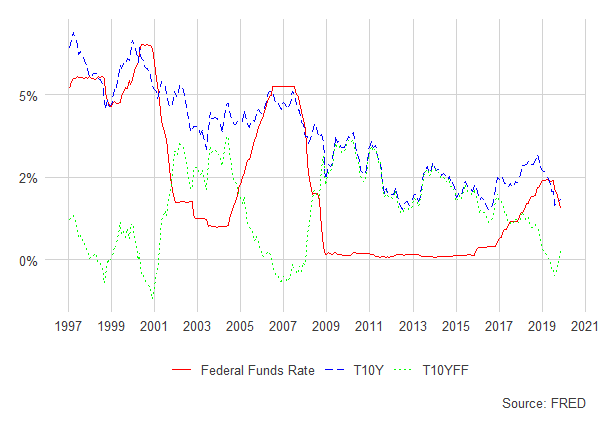
\includegraphics[width=0.8\textwidth]{mpmeasure.png}\\
T10Y is the 10 Year U.S. Treasury Bond Yield and 10YFF is the T10Y - Federal Funds Rate spread.
\label{fig:mpmeasure}
\end{figure}
\newpage
\subsection{Regression Results: Different Economic Periods}
\FloatBarrier
% Table created by stargazer v.5.2.2 by Marek Hlavac, Harvard University. E-mail: hlavac at fas.harvard.edu
% Date and time: Tue, Dec 10, 2019 - 2:18:54 AM
\begin{table}[h!] \centering 
  \caption{Time Robustness Checks for Fixed Effects Estimation} 
  \label{tbl8} 
\scriptsize 
\begin{tabular}{@{\extracolsep{5pt}}lcccc} 
\\[-1.8ex]\hline 
\hline \\[-1.8ex] 
 & \multicolumn{4}{c}{\textit{Dependent variable:}} \\ 
\cline{2-5} 
\\[-1.8ex] & \multicolumn{4}{c}{log(EMBI+ Spreads)} \\ 
\\[-1.8ex] & (1) & (2) & (3) & (4)\\ 
\hline \\[-1.8ex] 
 log(EFFR) & $-$0.130$^{***}$ & $-$0.162$^{***}$ & 0.583 & $-$0.281$^{***}$ \\ 
  & (0.023) & (0.023) & (6.487) & (0.026) \\ 
  GDP Growth & $-$2.997$^{***}$ & $-$2.865$^{***}$ & $-$2.283$^{***}$ & $-$1.642$^{***}$ \\ 
  & (0.274) & (0.294) & (0.421) & (0.279) \\ 
  CPI Inflation & 0.006$^{***}$ & 0.004$^{**}$ & 0.001 & 0.0002 \\ 
  & (0.001) & (0.002) & (0.001) & (0.003) \\ 
  Debt to GDP Ratio & 0.011$^{***}$ & 0.013$^{***}$ & 0.005$^{***}$ & 0.014$^{***}$ \\ 
  & (0.001) & (0.001) & (0.002) & (0.002) \\ 
  Deficit to GDP Ratio & $-$0.005 & $-$0.0002 & $-$0.021$^{***}$ & $-$0.009$^{*}$ \\ 
  & (0.004) & (0.004) & (0.007) & (0.005) \\ 
  REER & $-$0.008$^{***}$ & $-$0.009$^{***}$ & $-$0.009$^{***}$ & $-$0.013$^{***}$ \\ 
  & (0.001) & (0.001) & (0.001) & (0.001) \\ 
  Openness & 0.002$^{**}$ & 0.003$^{***}$ & $-$0.004$^{*}$ & $-$0.011$^{***}$ \\ 
  & (0.001) & (0.001) & (0.002) & (0.001) \\ 
  Credit Rating & 0.092$^{***}$ & 0.075$^{***}$ & 0.164$^{***}$ & 0.036$^{***}$ \\ 
  & (0.006) & (0.006) & (0.013) & (0.007) \\ 
  log(Reserves) & $-$0.111$^{***}$ & $-$0.123$^{***}$ & $-$0.219$^{***}$ & 0.024 \\ 
  & (0.022) & (0.024) & (0.046) & (0.020) \\ 
  log(VIX) & 0.636$^{***}$ & 0.527$^{***}$ & 0.652$^{***}$ & 0.247$^{***}$ \\ 
  & (0.027) & (0.028) & (0.045) & (0.026) \\ 
  Recession Dummy & $-$0.239 & $-$0.127 & $-$0.101 &  \\ 
  & (0.364) & (0.362) & (0.367) &  \\ 
  Great Recession Dummy & 0.191 & 0.192 &  &  \\ 
  & (0.365) & (0.363) &  &  \\ 
  Taper Dummy & 0.225$^{***}$ & 0.231$^{***}$ &  & 0.282$^{***}$ \\ 
  & (0.039) & (0.039) &  & (0.052) \\ 
  Lower Middle Income Dummy & $-$0.047 & 0.081 & 0.427 & $-$0.271$^{**}$ \\ 
  & (0.062) & (0.064) & (10.740) & (0.113) \\ 
  Upper Middle Income Dummy & 0.035 & 0.066 & 0.622 & 0.364$^{***}$ \\ 
  & (0.050) & (0.051) & (10.741) & (0.049) \\ 
  Lower Income Dummy & $-$3.648$^{***}$ & $-$3.009$^{***}$ & $-$2.070 &  \\ 
  & (0.463) & (0.411) & (10.750) &  \\ 
  log(EFFR)*Recession & 0.290 & 0.319 & 0.114 &  \\ 
  & (0.237) & (0.236) & (0.239) &  \\ 
  log(EFFR)*Great Recession & $-$0.301 & $-$0.324 &  &  \\ 
  & (0.238) & (0.236) &  &  \\ 
  log(EFFR)*Taper & 0.058$^{***}$ & 0.077$^{***}$ &  & 0.151$^{***}$ \\ 
  & (0.019) & (0.019) &  & (0.023) \\ 
  log(EFFR)*Lower Middle Income & 0.101$^{***}$ & 0.088$^{***}$ & $-$0.346 & 0.060$^{**}$ \\ 
  & (0.025) & (0.025) & (6.487) & (0.025) \\ 
  log(EFFR)*Upper Middle Income & 0.117$^{***}$ & 0.111$^{***}$ & $-$0.502 & 0.124$^{***}$ \\ 
  & (0.023) & (0.023) & (6.487) & (0.020) \\ 
  log(EFFR)*Lower Income & 2.366$^{***}$ &  & 1.275 &  \\ 
  & (0.278) &  & (6.493) &  \\ 
 \hline \\[-1.8ex] 
Observations & 3,306 & 3,047 & 1,434 & 1,539 \\ 
R$^{2}$ & 0.560 & 0.525 & 0.660 & 0.440 \\ 
Adjusted R$^{2}$ & 0.555 & 0.520 & 0.652 & 0.428 \\ 
\hline 
\hline \\[-1.8ex] 
\textit{Note:}  & \multicolumn{4}{l}{$^{*}$p$<$0.1; $^{**}$p$<$0.05; $^{***}$p$<$0.01} \\ 
 & \multicolumn{4}{l}{Specification (1) is the original fixed effects model.} \\ 
 & \multicolumn{4}{l}{Specification (2) estimates the model after the Asian Financial Crisis.} \\ 
 & \multicolumn{4}{l}{Specification (3) estimates the model before the Great Recession.} \\ 
 & \multicolumn{4}{l}{Specification (4) estimates the model after the Great Recession.} \\ 
 & \multicolumn{4}{l}{Standard errors are in parentheses.} \\ 
 \textit{Source:}& \multicolumn{4}{l}{author's calculations.} \\ 
\end{tabular} 
\end{table} 
\FloatBarrier

\subsection{Regression Results: Lagging Data}
\FloatBarrier
% Table created by stargazer v.5.2.2 by Marek Hlavac, Harvard University. E-mail: hlavac at fas.harvard.edu
% Date and time: Tue, Dec 10, 2019 - 4:13:07 AM
\begin{table}[!h] \centering 
  \caption{Lag Robustness Checks for Fixed Effects Estimation} 
  \label{tbl9} 
\scriptsize 
\begin{tabular}{@{\extracolsep{5pt}}lcccccc} 
\\[-1.8ex]\hline 
\hline \\[-1.8ex] 
 & \multicolumn{6}{c}{\textit{Dependent variable:}} \\ 
\cline{2-7} 
\\[-1.8ex] & \multicolumn{6}{c}{log(EMBI+ Spreads)} \\ 
\\[-1.8ex] & (1) & (2) & (3) & (4) & (5) & (6)\\ 
\hline \\[-1.8ex] 
 log(EFFR) & $-$0.032$^{***}$ & $-$0.035$^{***}$ & $-$0.030$^{***}$ & $-$0.018$^{**}$ & 0.011 & 0.056$^{***}$ \\ 
  & (0.006) & (0.007) & (0.007) & (0.008) & (0.008) & (0.008) \\ 
  GDP Growth & $-$3.126$^{***}$ & $-$3.329$^{***}$ & $-$3.482$^{***}$ & $-$3.427$^{***}$ & $-$2.720$^{***}$ & $-$2.921$^{***}$ \\ 
  & (0.276) & (0.313) & (0.334) & (0.351) & (0.365) & (0.381) \\ 
  CPI Inflation & 0.005$^{***}$ & 0.005$^{***}$ & 0.006$^{***}$ & 0.006$^{***}$ & 0.004$^{***}$ & 0.011$^{***}$ \\ 
  & (0.001) & (0.001) & (0.001) & (0.001) & (0.002) & (0.002) \\ 
  Debt to GDP Ratio & 0.010$^{***}$ & 0.010$^{***}$ & 0.012$^{***}$ & 0.013$^{***}$ & 0.013$^{***}$ & 0.006$^{***}$ \\ 
  & (0.001) & (0.001) & (0.001) & (0.001) & (0.001) & (0.001) \\ 
  Deficit to GDP Ratio & $-$0.004 & $-$0.005 & $-$0.008$^{*}$ & $-$0.017$^{***}$ & $-$0.033$^{***}$ & $-$0.021$^{***}$ \\ 
  & (0.004) & (0.005) & (0.005) & (0.005) & (0.005) & (0.006) \\ 
  REER & $-$0.008$^{***}$ & $-$0.007$^{***}$ & $-$0.004$^{***}$ & 0.0002 & 0.005$^{***}$ & 0.016$^{***}$ \\ 
  & (0.001) & (0.001) & (0.001) & (0.001) & (0.001) & (0.001) \\ 
  Openness & 0.002$^{***}$ & 0.003$^{***}$ & 0.004$^{***}$ & 0.004$^{***}$ & 0.006$^{***}$ & 0.011$^{***}$ \\ 
  & (0.001) & (0.001) & (0.001) & (0.001) & (0.001) & (0.001) \\ 
  Credit Rating & 0.093$^{***}$ & 0.090$^{***}$ & 0.076$^{***}$ & 0.051$^{***}$ & 0.022$^{***}$ & $-$0.019$^{**}$ \\ 
  & (0.006) & (0.006) & (0.007) & (0.007) & (0.008) & (0.008) \\ 
  log(Reserves) & $-$0.106$^{***}$ & $-$0.123$^{***}$ & $-$0.129$^{***}$ & $-$0.144$^{***}$ & $-$0.116$^{***}$ & $-$0.057$^{*}$ \\ 
  & (0.022) & (0.025) & (0.027) & (0.029) & (0.031) & (0.034) \\ 
  log(VIX) & 0.622$^{***}$ & 0.641$^{***}$ & 0.520$^{***}$ & 0.398$^{***}$ & 0.306$^{***}$ & 0.154$^{***}$ \\ 
  & (0.028) & (0.031) & (0.033) & (0.035) & (0.036) & (0.038) \\ 
  Recession Dummy & $-$0.271 & $-$0.034 & 0.180 & $-$0.246 & 1.083$^{**}$ & $-$1.560$^{***}$ \\ 
  & (0.371) & (0.421) & (0.448) & (0.471) & (0.488) & (0.487) \\ 
  Great Recession Dummy & 0.225 & 0.031 & $-$0.097 & 0.372 & $-$0.972$^{**}$ & 1.200$^{**}$ \\ 
  & (0.371) & (0.422) & (0.448) & (0.471) & (0.489) & (0.487) \\ 
  Taper Dummy & 0.217$^{***}$ & 0.215$^{***}$ & 0.127$^{**}$ & $-$0.041 & $-$0.321$^{***}$ & $-$0.702$^{***}$ \\ 
  & (0.037) & (0.044) & (0.051) & (0.062) & (0.082) & (0.267) \\ 
  log(EFFR)*Recession & 0.305 & 0.165 & 0.040 & 0.337 & $-$0.506 & 0.825$^{***}$ \\ 
  & (0.241) & (0.274) & (0.291) & (0.306) & (0.317) & (0.317) \\ 
  log(EFFR)*Great Recession & $-$0.316 & $-$0.113 & 0.112 & $-$0.059 & 0.918$^{***}$ & $-$0.819$^{***}$ \\ 
  & (0.242) & (0.275) & (0.292) & (0.307) & (0.318) & (0.317) \\ 
  log(EFFR)*Taper & 0.043$^{**}$ & 0.032 & 0.002 & $-$0.074$^{**}$ & $-$0.212$^{***}$ & $-$0.323$^{***}$ \\ 
  & (0.018) & (0.021) & (0.025) & (0.029) & (0.038) & (0.108) \\ 
 \hline \\[-1.8ex] 
Observations & 3,306 & 3,296 & 3,276 & 3,246 & 3,185 & 3,039 \\ 
R$^{2}$ & 0.543 & 0.482 & 0.415 & 0.354 & 0.290 & 0.176 \\ 
Adjusted R$^{2}$ & 0.539 & 0.477 & 0.409 & 0.348 & 0.283 & 0.167 \\ 
\hline 
\hline \\[-1.8ex] 
\textit{Note:}  & \multicolumn{6}{l}{$^{*}$p$<$0.1; $^{**}$p$<$0.05; $^{***}$p$<$0.01} \\ 
 & \multicolumn{6}{l}{Specification (1) is the original fixed effects model.} \\ 
 & \multicolumn{6}{l}{Specification (2) estimates the model with a 1 month lag.} \\ 
 & \multicolumn{6}{l}{Specification (3) estimates the model with a 3 month lag.} \\ 
 & \multicolumn{6}{l}{Specification (4) estimates the model with a 6 month lag.} \\ 
 & \multicolumn{6}{l}{Specification (5) estimates the model with a 1 year lag.} \\ 
 & \multicolumn{6}{l}{Specification (6) estimates the model with a 2 year lag.} \\ 
 & \multicolumn{6}{l}{Standard errors are in parentheses.} \\ 
 \textit{Source:}& \multicolumn{6}{l}{author's calculations.} \\ 
\end{tabular} 
\end{table} 
\FloatBarrier

\end{document}